\chapter{Motor modelling and control}\label{chap: modeling}
%
A widely used actuation system is reaction wheels which are spinning wheels and can exchange momentum with the spacecraft by increasing or decreasing the wheels speed. The rate of rotation can be adjusted by an electric motor and the magnitude of the wheels output torque is limited by the motors shaft torque. This chapter will provide characteristics of the chosen reaction wheels and BLDC motors along with the electrical and mechanical modelling of the motors for simulation purposes. 
%
\subsection*{Reaction wheels} \todo{merge with other reaction wheel section}
%
Since the focus of the current thesis is not on the design of reaction wheels, only few constraints are  taken into account for the selection of the wheels, such as the weight and the inertia. In order to minimize the total weight of the satellite, the weight of each wheel, is not overcome the weight of each motor. Furthermore, the chosen design gives higher inertia from the motor shaft, and can provide medium manoeuvrability in terms of time required to turn the satellite $90^o$ \cite{SIDI?}. The wheel inertia is \cite{flywheel design thesis} $J_{wheel} = 2.456 [gcm^2]$ and the weight is $w_{wheel} = 4.201 [g] $ compared to the motor weight $w_{motor} =8 [g] $ and the motor shaft inertia $J_{rotor} = 0.0249 [gcm^2]$  The characteristics of the selected motor can be found in \cite{chap: appendix}. The maximal speed of the motor is $\omega_{max}= 20000[rpm]$ and thus the maximum angular momentum that the system wheel-motor can provide can be found as \cite{SIDI}    
%
\begin{flalign*}
	h_{max} = {I_{wheel}} {\omega_{max}} 
\end{flalign*}
%0.000114450
which is found to be $4.2865*10^{-6} [Kgm^2/s]$ for each wheel.	
%
%
For 3 axis stabilization, 3 wheels each orthogonal to the principal axis, are enough but is not robust if one actuator fails. Redundancy is desired, requiring four or more wheels in positions oblique to all axis. The configuration of the wheels is chosen to be in tetrahedron shape since 4 reaction wheels system is more reliable and robust. The tetrahedron configuration will be discussed in an other chapter.  
\subsection*{BLDC motor model}
%

In order to make the system more reliable, brush-less DC motors are chosen as actuators. BLDC motors are lighter compared to brushed with the same power output and do not causing sparking thus can be used in operations that demand long life and reliability.
%
Each motor consists of an electrical part and a mechanical part. The electrical part of the motor can be modelled using Kirchhoff's Voltage Law as
%
\begin{flalign}
 V_{a} -V_{R}-V_{L} -V_{e} = 0
\label{Kirchhoff1}
\end{flalign}
%
where $V_{a}$ is the voltage source, $V_{R}$ is the voltage drop across the resistance, $V_{L}$ is the voltage drop across the inductance and $V_{e}$ is the back emf. \Eqref{Kirchhoff1} can be re written as 
%
\begin{flalign}
	V_{a}= R_{a}i + L_{a}\dfrac{di}{dt}+ k_{e}\omega
	\label{Kirchhoff244}
\end{flalign}
%
 where $R_{a}$ [Ohm] is the armature resistance, $L_{a}$ [H] is the armature inductance and $k_{e}$ is the back emf coefficient as it can be seen in the \figref{fig:electromech} .   
%
\begin{table}[H]
	\begin{minipage}[b]{0.49\linewidth}
		\centering
		\begin{figure}[H]
			\centering
			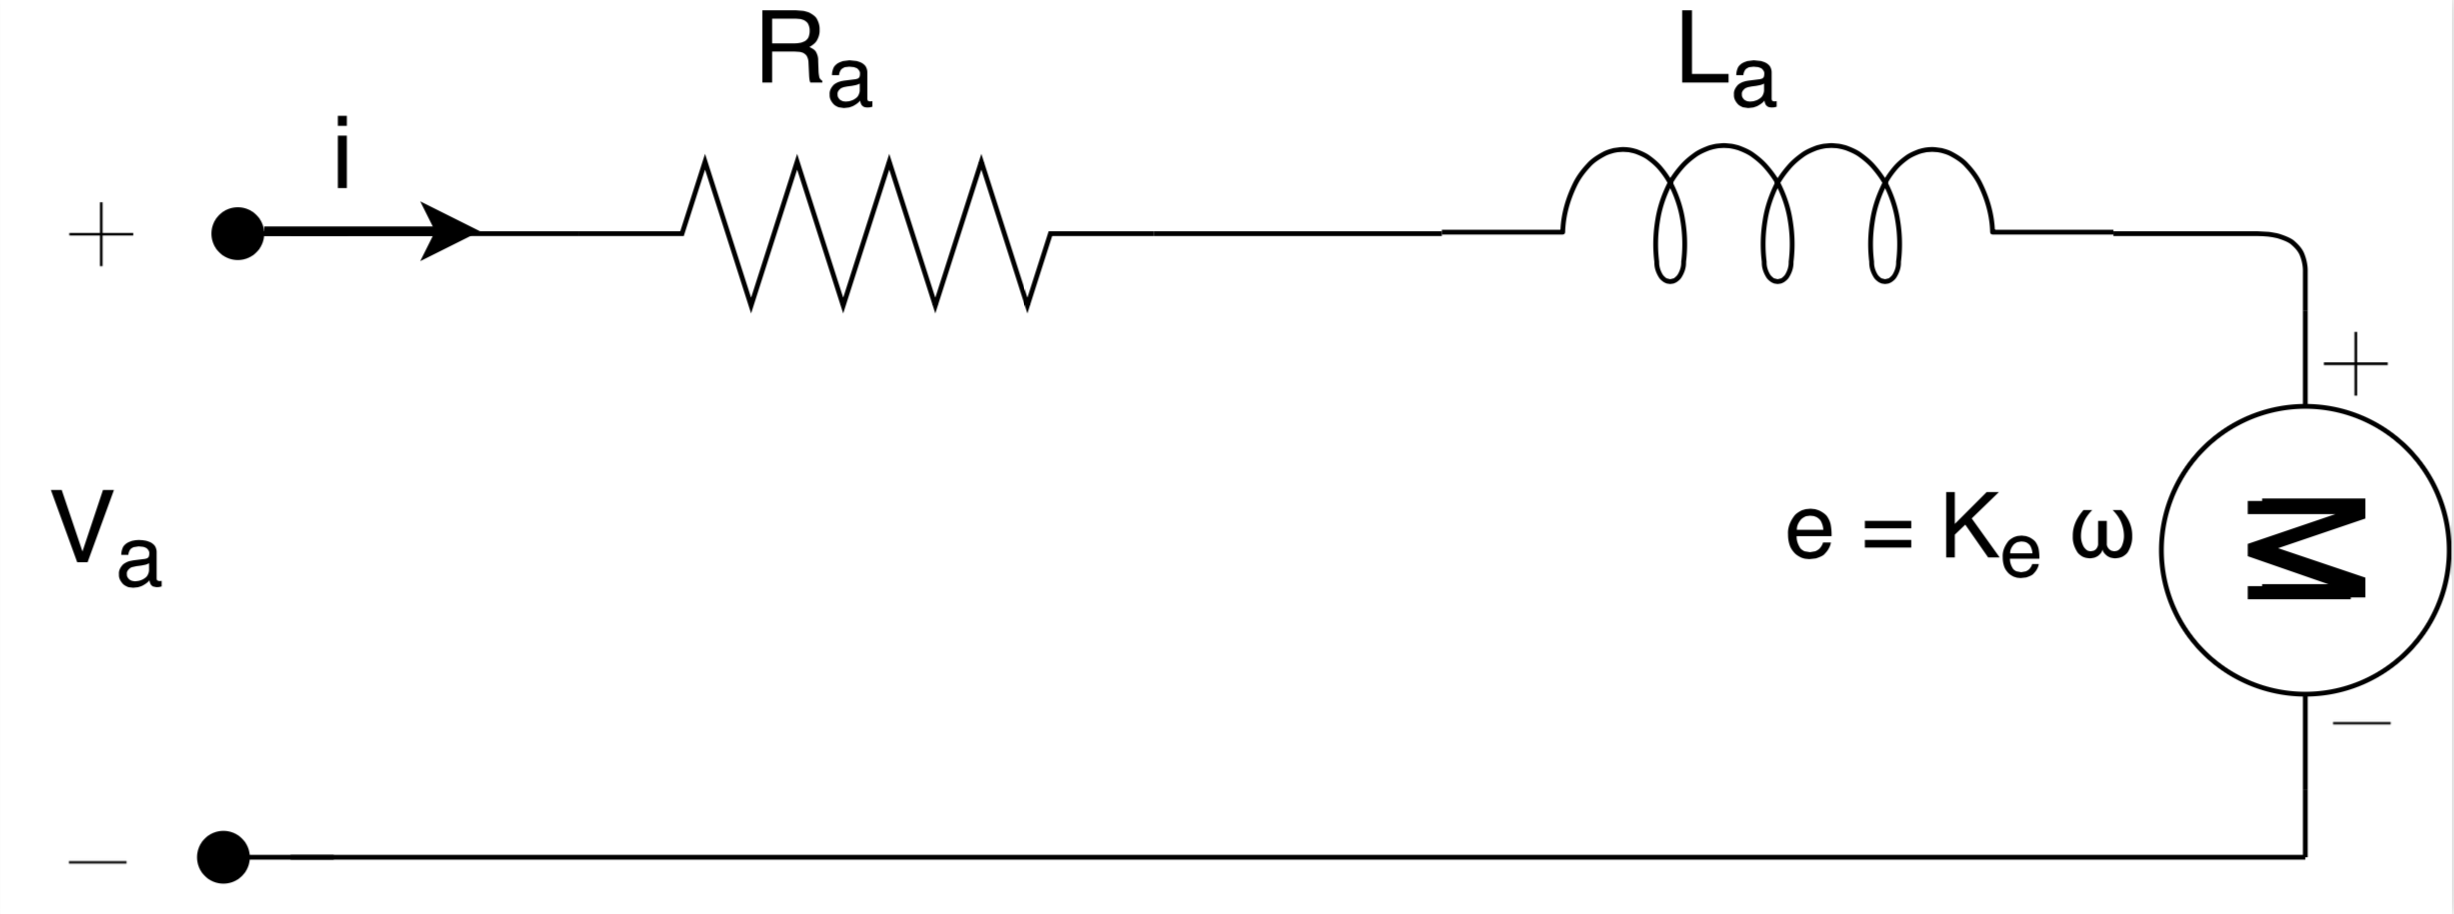
\includegraphics[width=1\linewidth]{figures/BLDC}
			%\caption{ Electrical and mechanical part of the motor }
		%	\label{fig:electromech}
		\end{figure}
	\end{minipage}\hfill
	\begin{minipage}[b]{0.49\linewidth}
		\centering
		\begin{figure}[H]
			\centering
			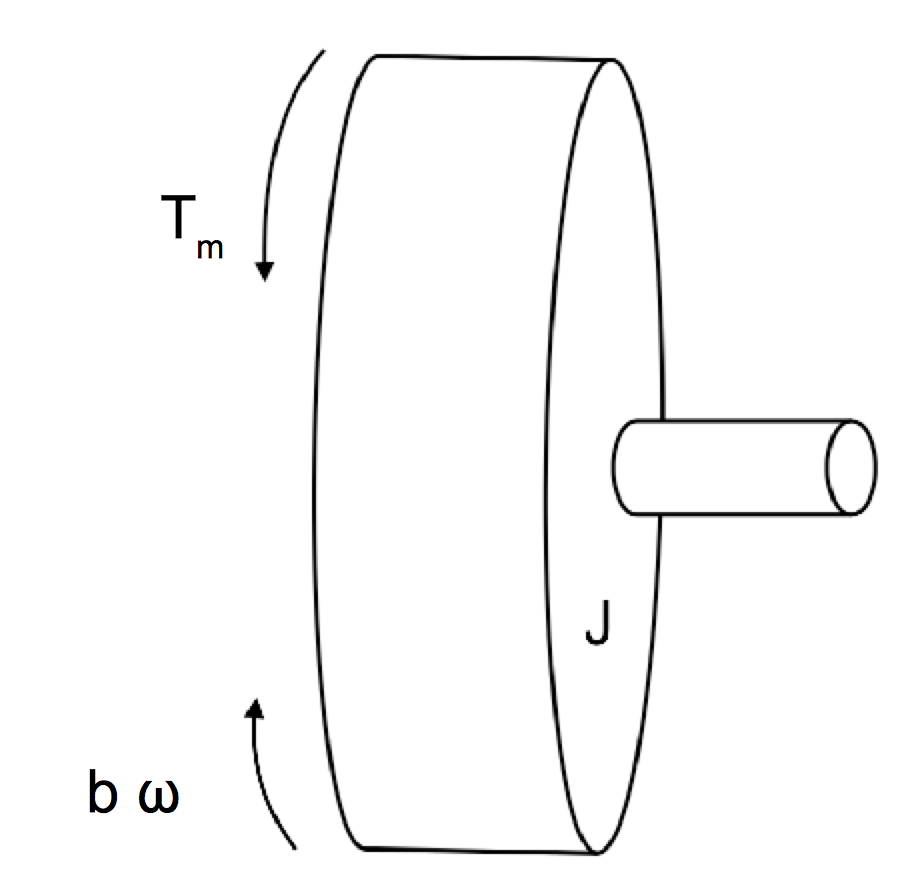
\includegraphics[width=0.55\linewidth]{figures/flywheel_1}
			%\caption{Mechanical part of the motor}
			%\label{fig:distancecontrol4}
		\end{figure}
	\end{minipage}
	\caption{ Electrical and mechanical part of the motor }
	\label{fig:electromech}
\end{table}

%
The mechanical part of the motor can be modelled as 
%
\begin{flalign}
 k_{t}i  =J\dfrac{d\omega}{dt} + b\omega
	\label{mechpart66}
\end{flalign}
%
where $J$ is the rotor moment of inertia, $k_{t}$ [Nm/A] is the motor torque coefficient and $b$ [Nm s/rad] is the viscous friction coefficient. Assuming the current will not increase rapidly in order not to harm the equipment, and moreover the electrical time constant $\tau_{e}=\dfrac{L}{R}$ is much smaller than the mechanical time constant $\tau_{m}=\dfrac{J}{b}$, the effect of the inductance can be neglected and the \eqref{mechpart66} can be solved for $i$ and  replaced in \eqref{Kirchhoff244}\cite{permanent magnet}     
%
\begin{flalign}
	i  =\dfrac{J}{k_{t}}\dfrac{d\omega}{dt} + \dfrac{b}{k_{t}}\omega
	\label{mechpart2}
\end{flalign}
%
\begin{flalign}
\dfrac{RJ}{k_{t}}\dfrac{d\omega}{dt}+\dfrac{Rb}{k_{t}}\omega +k_{e}\omega = V_{a}
	\label{mechpart333}
\end{flalign}
%
by laplace transformed \eqref{mechpart333}, the first order transfer function from $V_{a}$ to $\Omega$ can be written as 
%
\begin{flalign}
	\dfrac{\Omega(s)}{V_{a}(s)}= \dfrac{\dfrac{k_{t}}{Rb+k_{e}k_{t}}}{\dfrac{RJ}{Rb+k_{e}k_{t}}s+1}
	\label{tf}
\end{flalign}
%
the block diagram of the system can be seen in \figref{fig:blockdi} where $\tau_{me} = \dfrac{RJ}{Rb+k_{e}k_{t}} $ is the time constant of the first order system for each motor. For four wheels, four motors are used in tetrahedron configuration. The total moment of inertia of the motor-wheel system is the sum of individual moments $J = J_{wheel}+J_{rotor}$. Since $J_{wheel}\gg J_{rotor}$ the inertia of the rotor can be neglected.
%
\begin{figure}[H]
	\centering
	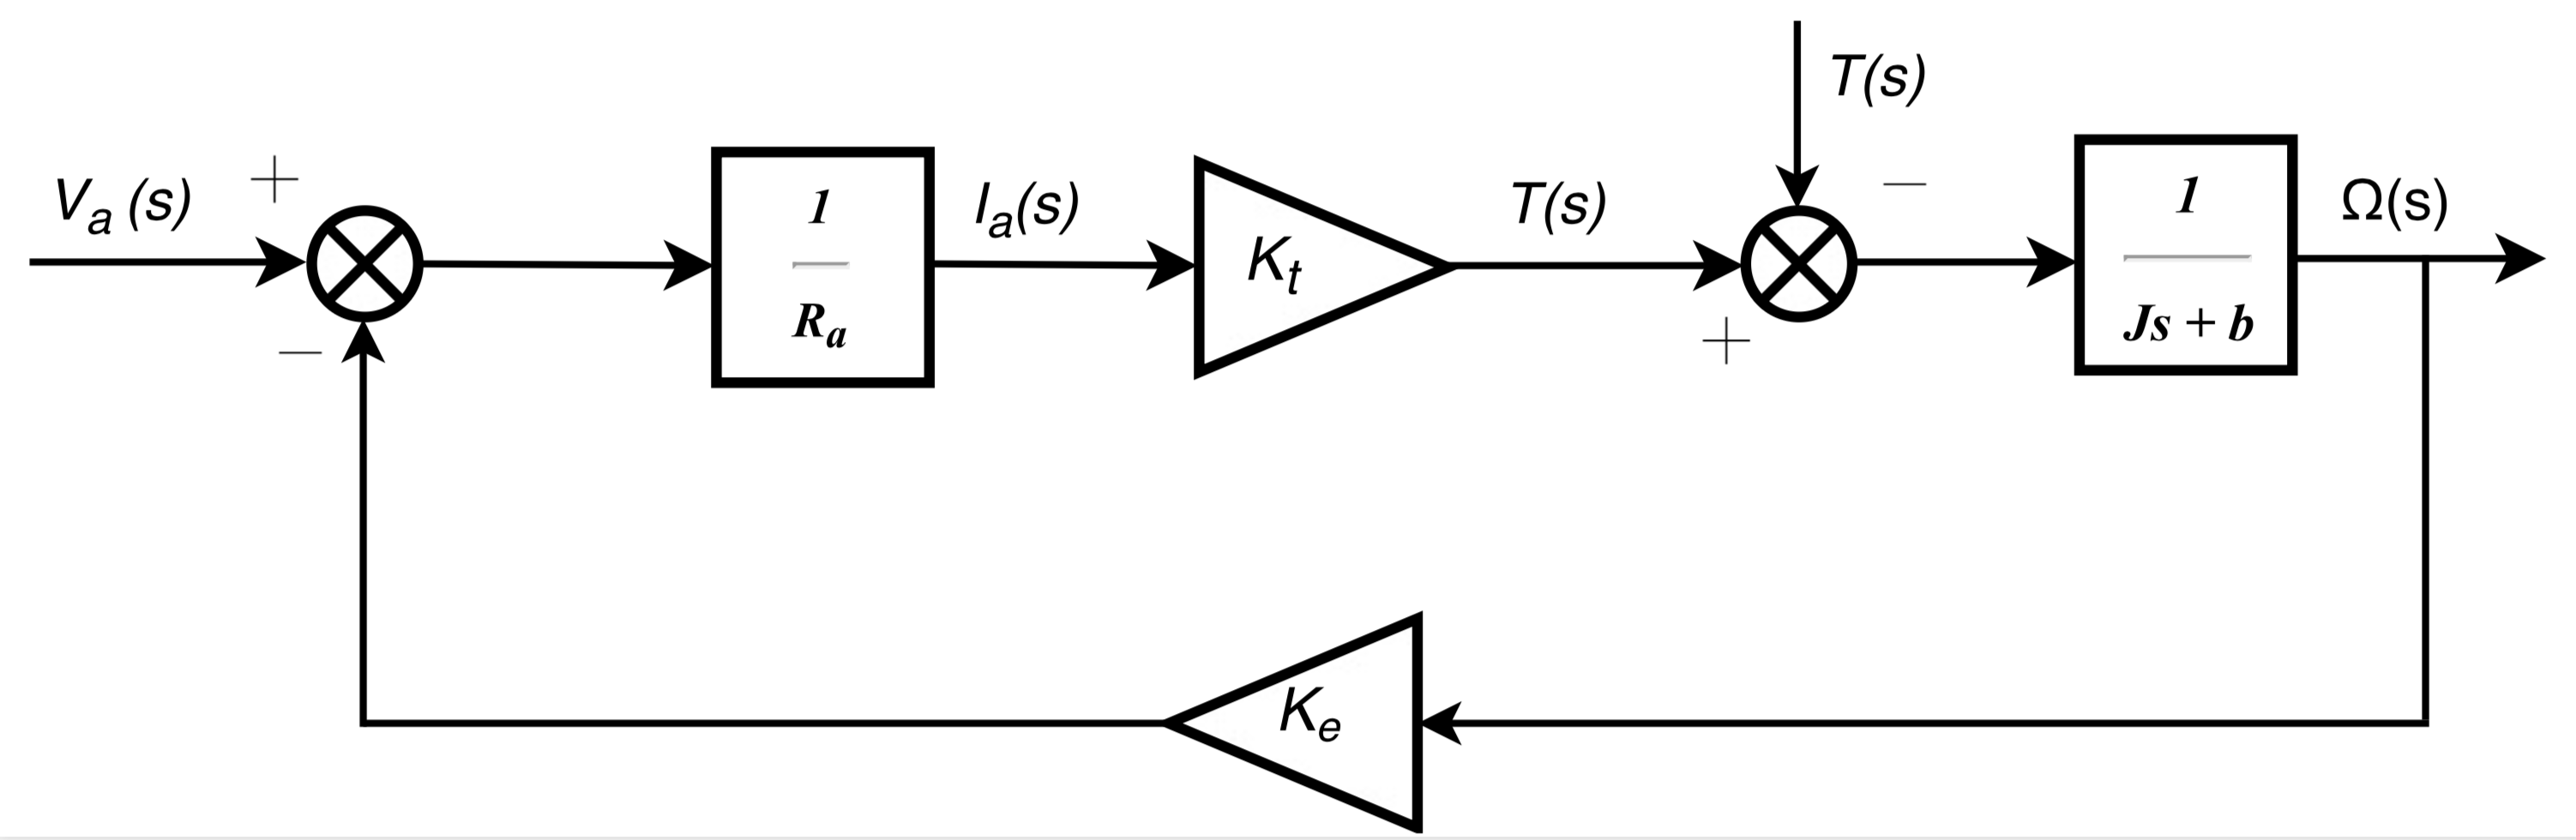
\includegraphics[width=0.7\linewidth]{figures/block_diagram_1}
	\caption{Block diagram of the motor system}
	\label{fig:blockdi}
\end{figure}
%
\subsection*{Motor control}
 \todo{more details about previous work}
In previous work, two controllers a linear and a non-linear(SMC), have been designed requiring a torque that has to be produced from the motors-wheel system. This torque demand is used to give the desired angular velocity reference for the wheels and thus the torque that will be fed back to the satellite as seen in the \cite{block diagram}. The output torque from the linear and non-linear controllers has three elements which has to be transformed in the tetrahedron configuration using the matrix \eqref{tetrahedron}  A PI controller has been designed to control the angular velocity of the motor as seen in the \figref{fig:blockdi222} .
\\
\begin{figure}[H]
	\centering
	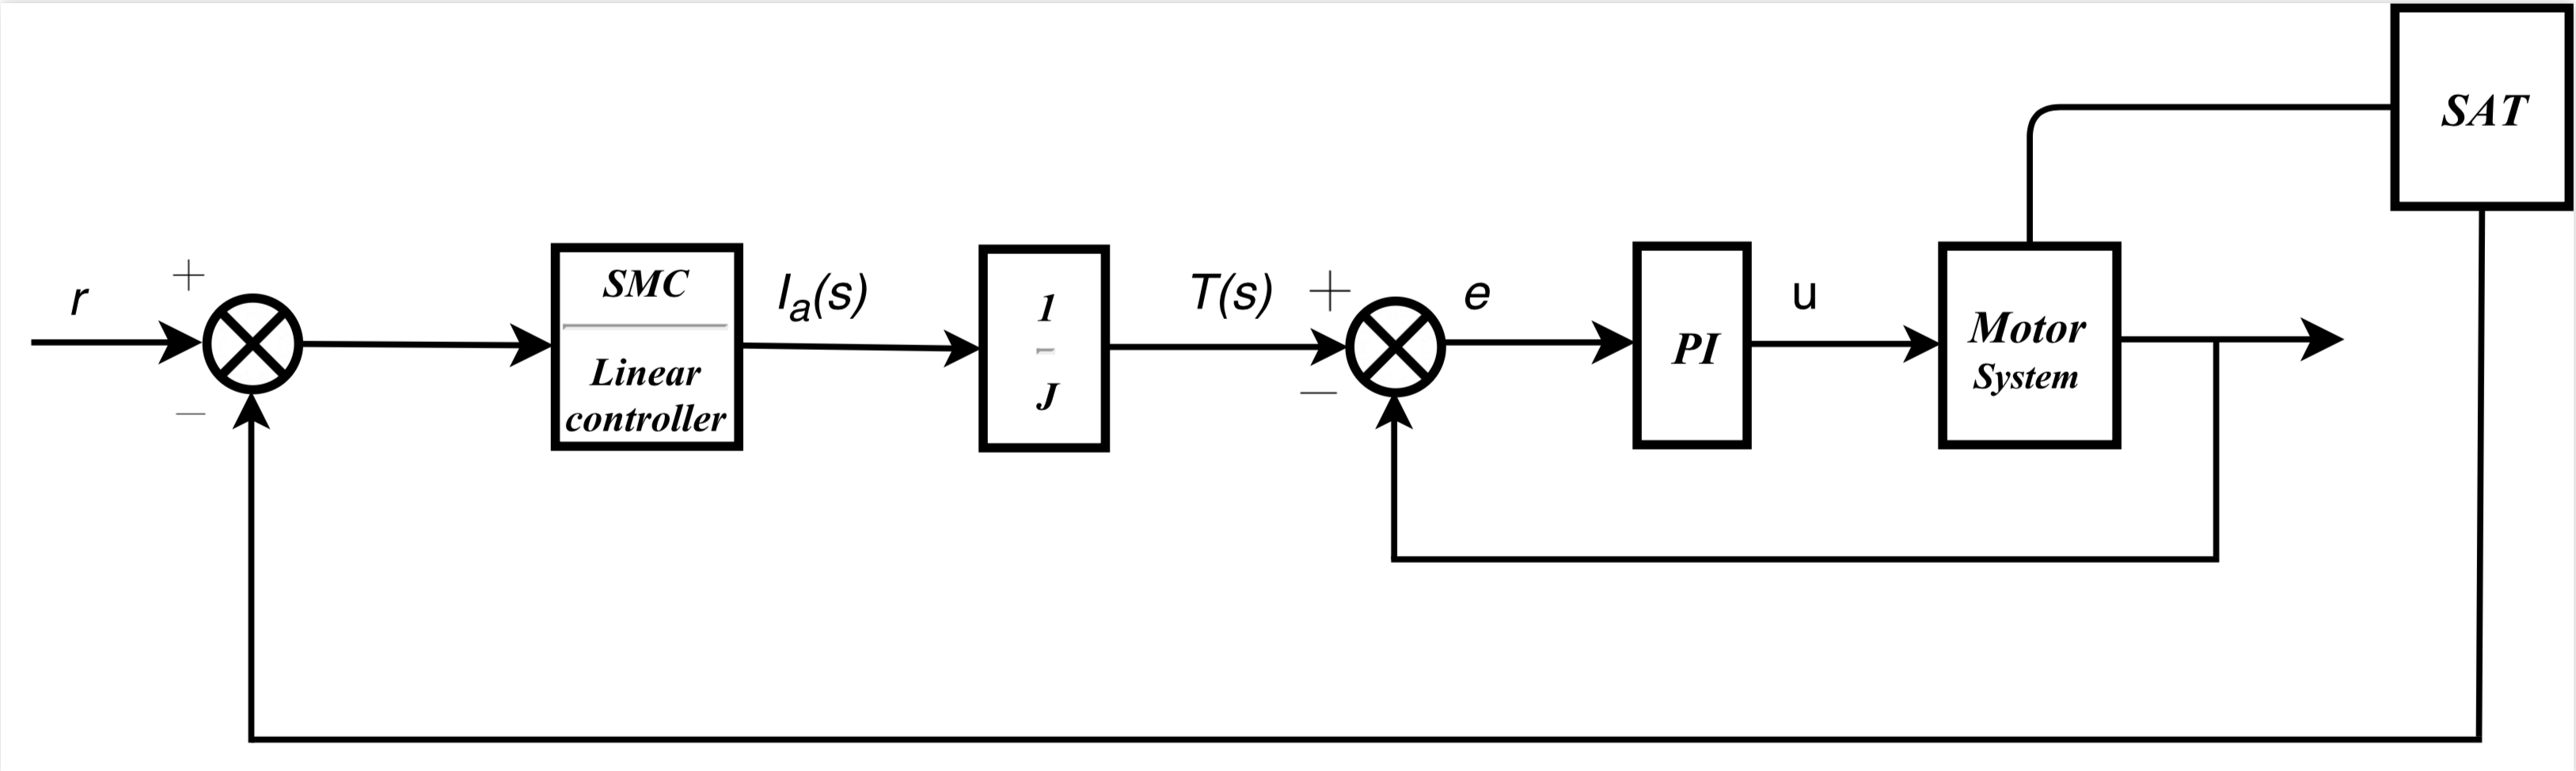
\includegraphics[width=0.7\linewidth]{figures/block_diagram_2}
	\caption{Block diagram of the motor control with PI controller WE HAVE TO CHANGE THE FIGURE}
	\label{fig:blockdi222}
\end{figure}  
%
The PI controller gains are chosen based on the open loop system response using the Ziegler-Nichols method \cite{PID tuning} and by trial and error in order to achieve faster closed loop response and asymptotically stable system. The gains are chosen to be   
%
\begin{flalign*}
	k_{p} = 3.4 \\ k_{i} = 0.9
\end{flalign*}
% 
\todo{make figure bigger}
The root locus of one motor with PI controller is seen in the \figref{fig:rlocus33}
%
\begin{figure}[H]
	\centering
	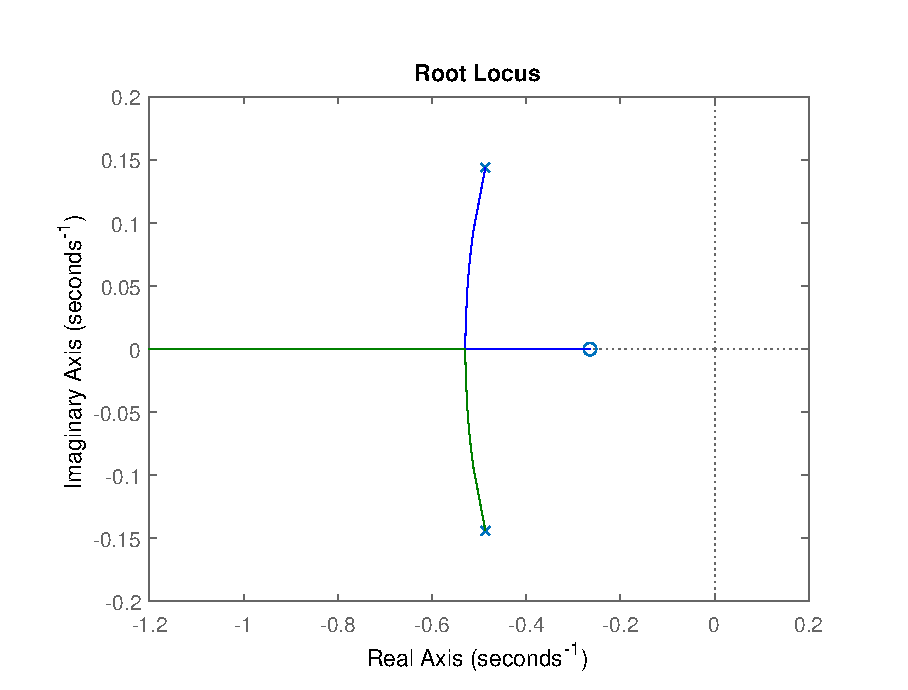
\includegraphics[width=0.7\linewidth]{figures/pid_rootlocus}
	\caption{Root locus of one motor with PI controller}
	\label{fig:rlocus33}
\end{figure}
%
The closed loop system gives complex eigenvalues and fast response and is stable for a wide range of the adjustable parameters. 
%

%
\chapter {Environmental disturbance torques}
  \label{chap: distTorques}
%
Disturbance torques can be classified either as external or internal \todo{dont distuingish between external and internal}. Since the external disturbances are larger in magnitude compared to \todo{reference} internal and can cause a change in the total momentum of the spacecraft, only these will be accounted. The external disturbing torques that will be discussed are aerodynamic, solar radiation and gravity gradient torque.
\subsection*{Aerodynamic disturbance torque}\label{chap: disturbances}
%
Gas molecules, in a LEO(low Earth orbit) collide with the surface of the satellite causing
a force which direction opposes the direction of the satellites velocity vector. This Aerodynamic force can be modelled as \cite{SADC,our report}  


\begin{flalign}
	\vec{F_A} = -\frac{1}{2} \rho \ C_D \ A_{\perp}   \vec{v}^2
	\label{eq:ec1c}
\end{flalign}

where $\rho$ is the atmospheric density  
is chosen to be constant and equal to $1.454 \cdot 10^{-13} Kg/{m^3}$ based on the Committee on Space Research\cite{FSA}, $\vec{v}$ is the satellite velocity vector, $A_{\perp}$ is the area perpendicular to the velocity and $C_D$ is the drag coefficient and is usually chosen to be equal to 2 \cite{SADC}\cite{our report}  . If the calculation of the lifetime of the satellite is of great importance a more accurate drag coefficient should be used.

Using the \eqref{eq:ec1c}, the aerodynamic torque acting on the satellite can be written as 
\begin{flalign}
	\vec N_{drag} = \vec r_{s} \times  \vec F_{A} 
	\label{eq:drag}
\end{flalign}
where:\\
$\vec r_{s}$ is the vector from the centre of mass of the satellite to the geometric centre of the exposed area\\
\subsection*{Solar radiation disturbance torque}\label{chap: disturbances2}

Solar radiation pressure is emitted from various sources such as reflection from the Earth's atmosphere, from solar wind and direct radiation from the sun to the surface of the satellite\cite{SADC}\cite{our report}  . Direct radiation is larger and only this source will be taken into account.

The solar flux is given as
\begin{flalign}
	P = \dfrac{F_s}{c}
	\label{eq:flux2}
\end{flalign}

where $F_s$ is the intensity or mean energy flux given as 1358 [$W/m^2$] and $c$ is the speed of light. The solar radiation force $\vec F_{rad}$ can be expressed as 

\begin{flalign}
	\vec {F_{rad}} = C_{a} P A \ \hat{S}
	\label{eq:Pres}
\end{flalign}
where $C_{a}\in [0,2]$ is the absorption coefficient which depends on the material of the satellite with 2 \todo{decide if 1.5 or 2 should be used} be the value of totally reflected beam, $P$ is the solar flux, $A$ is the radiated surface area, and $\hat{S} =\frac{\vec {r_{sun,sat}}}{||\vec {r_{sun,sat}}||}$ is the unit vector from the satellite to the sun. The solar radiation torque can be computed as 
\begin{flalign}
	\vec N_{drag} = \vec r_{s} \times  \vec F_{rad} 
	\label{eq:solar}
\end{flalign}
where $\vec r_{s}$ is the vector from the center of mass of the satellite to the center of pressure.
%
\subsection*{Gravity Gradient disturbance torque and $J_2$  perturbation}\label{chap: disturbances3} \todo{separate}
%
Due to the non spherical mass distribution and non homogeneity of the Earth, a pertubative gravitational force($J_{2}$ perturbation)\cite{SADC}\cite{our report} exerted on the satellite determining its orbit difference compared to ideal mathematical models.
Contrary to this, in order to derive an expression for the gravitational torque exerted about the mass centre of the satellite, it will be assumed symmetrical, spherical distribution of the Earth's mass\cite{SADC} with this assumption be valid by comparing the magnitude of the gravity gradient with the other pertubative torques.     
\subsubsection{$J_2$ gravity perturbation}
An approximation of the gravitational potential of the Earth is \cite{SADC}\cite{our report}:
\begin{flalign}
	U \approx -\frac{\mu}{r} \left[1 - \sum_{n=2}^{\infty} \left(\frac{R_e}{r}\right)^{n} J_n P_n sin(\phi)  \right ] = \frac{\mu}{r} [U_0 + U_{J_2} + U_{J_3} + ...]
	\label{eq:Pr341}
\end{flalign}
which has been derived using the spherical harmonic expansion describing deviations of the potential to the south and north direction,
with $U_0$ = -1, $U_{J_2}$ = $\left(\frac{R_e}{r}\right)^{2} J_2 \frac{1}{2} (3 sin^2 \phi -1) $ and ${J_2}$ be a numerical coefficient, with the other terms been discarded.

The final relation is obtained as 
\begin{flalign}
	\vec F = -m \nabla U
	\label{eq:Pr3431}
\end{flalign}
with the vector $\vec F$ expand to the components \cite{SIDI}\cite{our report}  :
\begin{flalign}
	F_x = -\frac{\partial U}{\partial x} = \mu \left[ -\frac{x}{r^3} + A_{J_2} \left(15 \frac{xz^2}{r^7} - 3\frac{x}{r^5}   \right ) \right ]       \\
	F_y = -\frac{\partial U}{\partial y} = \mu \left[ -\frac{y}{r^3} + A_{J_2} \left(15 \frac{yz^2}{r^7} - 3\frac{y}{r^5}   \right ) \right ]       \\
	F_z = - \frac{\partial U}{\partial z} =  \mu \left[ -\frac{z}{r^3} + A_{J_2} \left(15 \frac{z^3}{r^7} - 3\frac{z}{r^5}   \right )  \right]       
	\label{eq:Pr34331}
\end{flalign}
where $A_{J_2}  = \frac{1}{2} J_2 R_e^2$ and and $R_e$ is the mean radius o the Earth at the equator
%
%
\subsubsection{Gravity-Gradient torque}
The gravity gradient effect about the centre of mass of the satellite is a consequence of the non uniform gravitational field of the Earth. The torque about the centre of mass of the satellite can be expressed as\cite{SADC}\cite{our report}  
%
\begin{flalign}
	\vec N_{gra} &= \dfrac{3\mu}{\vec R_{sc}^3}[\vec{\hat R_{sc}} \times(\vec{I} \ \vec{\hat R_{sc}}] 
	\label{eq:ref4}
\end{flalign}
where $\vec{\hat R_{sc}}$ is the unit vector from geometric centre of the earth's to the satellite's geometric centre, $\mu = G*m_{earth}$ with $G$ be the Gravitational constant $6.6740*10^{-11}$ [$m^{3} kg^{-1} s^{-2}$] and $\underline I$ is the inertia matrix of the satellite. 